\begin{summary}
    \begin{center}
        \begin{tabular}{ll}
            \toprule
            \textbf{Concepts} & \textbf{Description} \\
            \toprule
            \textbf{Math symbols} & \\
            \multicolumn{2}{p{\linewidth}}{
            \begin{itemize}
                \item \(x, y, b, h, z\) - Vectors (input, outputs, bias, hidden, latent)
                \item \(\hat{y}\) - Predictions
                \item \(\theta\) - Parameters (collections of tensors)
                \item \(f, f_i, f_j, C\) - Functions
                \item \(x_i\) - Scalar, \(i\)-indexed coordinate of \(x\)
                \item \(X, W\) - Matrices
                \item \(\frac{\partial f}{\partial x_i}\) - Partial derivative of \(f\) with respect to \(x_i\)
                \item \(\nabla f\) - Gradient of \(f\)
            \end{itemize}} \\
            \midrule
            \textbf{Hyperparameter choices} & \\
            \multicolumn{2}{p{\linewidth}}{
                \begin{center}
                    \customFigure[0.5]{../Images/L3_12.png}{}
                    \vspace{-4em}
                \end{center}} \\
            \midrule
            \textbf{Finding the best parameters} & Minimize the error b/w predictions and actual values. \\
            & $ C(\theta) = \sqrt{\frac{1}{N} \sum_n (y_n - f(x_n; \theta))^2} = \text{RMSE}(y, f(x; \theta))$ \\ 
            \midrule
            \textbf{Gradient Descent: Rolling Down Hill} & Update rule to iteratively adjust parameters to reduce loss. \\
            & $\theta_n = \theta_{n-1} - \alpha \nabla C(\theta_{n-1})$ \\
            \multicolumn{2}{p{\linewidth}}{
                \begin{itemize}
                    \item \textbf{Notes:} Multiple minima, gradient info (sign (\textcolor{green}{+}, \textcolor{red}{-}), magnitude), initialization matters, learning rate $\alpha$. 
                    \customFigure[0.3]{../Images/L3_3.png}{}
                \end{itemize}} \\
            \bottomrule
        \end{tabular}
    \end{center}
\end{summary}
\newpage

\begin{summary}
    \begin{center}
        \begin{tabular}{ll}
            \toprule
            \textbf{Concepts} & \textbf{Description} \\
            \midrule
            \textbf{Backprop: Forward and Backward Passes} & Calculating predictions, tracking operations, and computing gradients. \\
            \multicolumn{2}{p{\linewidth}}{
                \begin{itemize}
                    \item 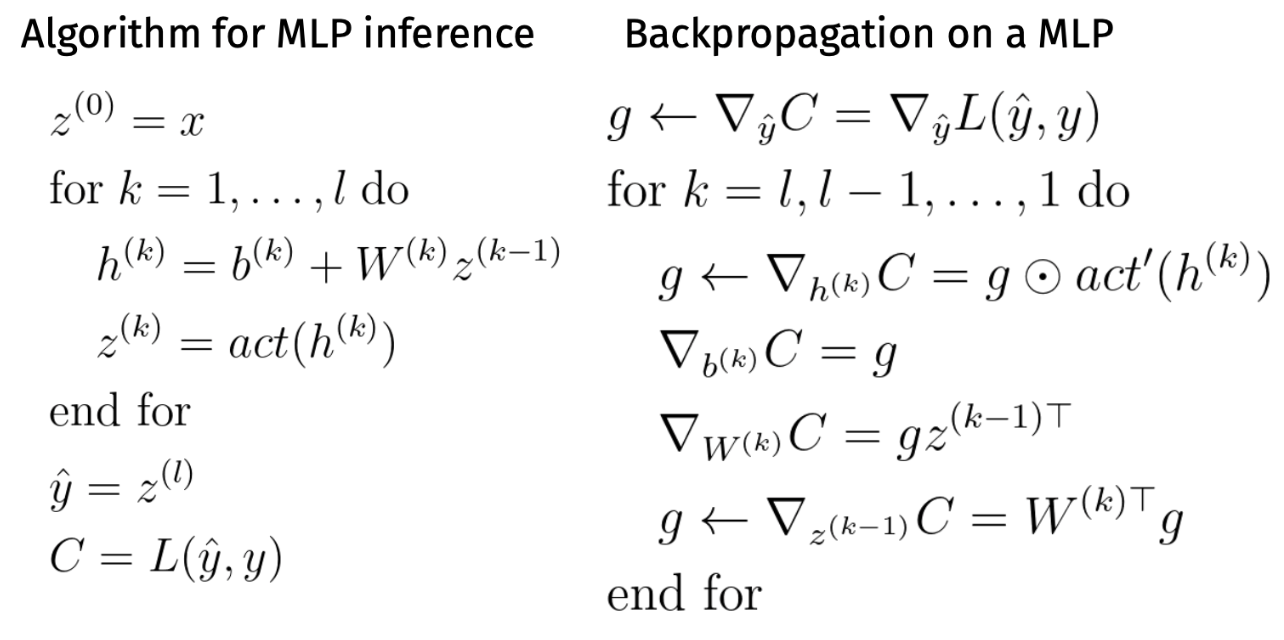
\includegraphics[width=0.5\linewidth]{../Images/L3_13.png}
                    \item $g \leftarrow \nabla_{\hat{y}} C = \nabla_{\hat{y}} L(\hat{y}, y)$: Compute gradient on output layer.
                    \item $g \leftarrow \nabla_{h^{(k)}} C = g \odot \text{act}'(h^{(k)})$: Convert gradient on layer output into a gradient on the pre-nonlinearity activation.
                    \item $\nabla_{b^{(k)}} C = g$: Compute gradient on biases.
                    \item $\nabla_{W^{(k)}} C = g z^{(k-1)\top}$: Compute gradient on weights.
                    \item $g \gets \nabla_{z^{(k-1)}} C = W^{(k)\top} g$: Propagate gradients w.r.t. the next lower-level activations.
                \end{itemize}
            } \\
            \midrule
            \textbf{Inductive Bias (Learning Bias)} & Set of assumptions that the learner applies to a model for a task, \\
            & guiding the learning process towards specific patterns. \\ 
            \midrule
            \textbf{MLE} & Choosing parameters that maximize the likelihood (probability) \\
            & of observing the given data. \\
            \multicolumn{2}{p{\linewidth}}{
                \begin{itemize}
                    \item \textbf{Notes:} Minimizing negative log-likelihood results in loss functions.
                \end{itemize}
            } \\
            \midrule
            \textbf{Useful Trick in DL} & Transforming smoothly Gaussian-like data into Non-Gaussian data \\
            & using Linear Transforms + Activations. \\
            \multicolumn{2}{p{\linewidth}}{
                \begin{itemize}
                    \item \textbf{Differentiable tools:} relu, sum, mean, var, softplus, sigmoid, softmax, masking.
                    \item \textbf{Non-differentiable:} argmax, top-k, binarize.
                \end{itemize}
            } \\
            \midrule
            \textbf{Regression - Gaussian Distribution} & Likelihood estimation for regression models. \\
            \multicolumn{2}{p{\linewidth}}{
                \begin{itemize}
                    \item \textbf{Likelihood:} The probability density of observing the actual output values given the inputs and model parameters.
                    \item \textbf{MLE:} Minimizing negative log-likelihood leads to the Mean Squared Error.
                    \item \textbf{Activation Function:} $\text{Act} = x$: Identity function.
                \end{itemize}
            } \\
            \bottomrule
        \end{tabular}
    \end{center}
\end{summary}

% \begin{example}
%     \begin{itemize}
%         \item \textbf{Why should the transformation be differentiable?} 
%         \begin{itemize}
%             \item Smooth
%         \end{itemize}
%     \end{itemize}    
% \end{example}

\subsubsection{Regression - Gaussian Distribution}
\begin{notes}
    \begin{itemize}
        \item \textbf{Likelihood:} The probability density of observing the actual output values given the inputs and our model parameters (weights, bias, and the variance of the noise).
        \item \textbf{MLE:} Minimizing negative Log-Likelihood leads to the Mean Squared Error:
        \[
        \frac{1}{n} \sum_n (y_n - \hat{y}_n)^2
        \]
        \item \textbf{Activation Function:} $\text{Act} = x$: Identity function.
    \end{itemize}
    \customFigure[0.5]{../Images/L3_4.png}{}
\end{notes}

\subsubsection{Masking: Omit data when missing or NA}
\begin{notes}
    Multiply loss function by a binary valued mask. 
    \begin{equation*}
        \frac{1}{\sum \text{mask}} \sum_n \text{mask}_n \cdot (y_n - \hat{y}_n)^2
    \end{equation*}
    \begin{itemize}
        \item Good for NaN, $-\infty$, high value outliers.
    \end{itemize}
    \customFigure[0.5]{../Images/L3_5.png}{}
\end{notes}

\subsubsection{Binary Classification - Binomial Distribution}
\begin{notes}
    \begin{itemize}
        \item \textbf{Likelihood:} The probability of observing the actual class labels (0 or 1) given the inputs and our model parameters.
        \item \textbf{MLE:} Minimizing negative Log-Likelihood leads to the Binary Cross Entropy loss (BCE):
        \[
        \frac{1}{n} \sum_n \left( y_n \log(\hat{y}_n) + (1 - y_n) \log(1 - \hat{y}_n) \right)
        \]
        \item \textbf{Activation Function:} $\text{Act} = \text{sigmoid}$: Squashes the output to $[0, 1].$
    \end{itemize}
    \customFigure[0.5]{../Images/L3_6.png}{}    
\end{notes}

\subsubsection{Multilabel Classification - N-dim Binomial Distribution}
\begin{notes}
    \begin{itemize}
        \item \textbf{Loss function:} \textbf{Sum} of Binary Cross Entropy (BCE) for each label:
        \[
        \frac{1}{n} \sum^{\text{labels}} \sum_n \left( y_n \log(\hat{y}_n) + (1 - y_n) \log(1 - \hat{y}_n) \right)
        \]
        \item \textbf{Activation Function:} $\text{Act} = \text{sigmoid}$: Squashes the output to $[0, 1].$
    \end{itemize}
    \customFigure[0.5]{../Images/L3_7.png}{}        
\end{notes}

\subsubsection{Multiclass Classification - Multinomial Distribution}
\begin{notes}
    \begin{itemize}
        \item \textbf{Loss function:} Cross entropy (CE):
        \[
        \sum_{\text{classes } i} y_i \log(\hat{y}_i)
        \]
        \item \textbf{Activation Function:} $\text{Act} = \text{softmax}$, where $\text{softmax}(z) = \frac{e^{z_i}}{\sum_j e^{z_j}}$
    \end{itemize}
    \customFigure[0.5]{../Images/L3_8.png}{}
\end{notes}

\subsubsection{Ordinal Classification}
\begin{notes}
    \begin{itemize}
        \item \textbf{Activation Function:} $\text{Act} = \text{sigmoid}$
    \end{itemize}
    \customFigure[0.5]{../Images/L3_9.png}{}
\end{notes}

\subsubsection{Zero-Inflated Distribution}
\begin{example}
    \[
    \text{Pred}(z) =
    \begin{cases}
        \text{active}: \text{sigmoid}(W_b \cdot z) \\
        \text{value}: W_r \cdot z
    \end{cases}
    \]

    \[
    \text{BCE}(\text{mask}, y_{\text{pred,binary}}) + \text{mask} \cdot * \text{MSE}(y_{\text{true}}, y_{\text{pred,reg}})
    \]
    \customFigure[0.75]{../Images/L3_11.png}{}
\end{example}
